\chapter{State of the Art}
\label{state_of_the_art}

In this chapter we will present the state of the art on the field of modular robotics. More precisely, we will discuss the state of the art of the main modules used in modular robotics research, from which we took inspiration to design our platform; the state of the art of the controllers used for achieving locomotion on chain-type modular robots and the state of the art of modular robotics communications.\\


\section{Modular Robotic Platforms}
\label{state_art_modules}
This section summarizes the current development in modular robotics, showing the most significant modules in the field, as well as the most related to the design developed by the author, and presented in chapter \ref{hardware_chapter}.

%%%% PolyPod %%%%%%%%%%%%%%%%%%%%%%%%%%%%%%%%%%%%%%%%%%%%%%%%%%%%%%%%%%%%%%
\subsection{PolyPod}
\label{state_modules_PolyPod}

PolyPod \cite{Yim1994, Yim1993} is a modular robot created by Mark Yim in 1994 for his PhD thesis, and can be considered the first robot created with the modular robotic paradigm in mind.\\

PolyPod is a heterogeneous system made of two different types of modules, called ``segments'' and ``nodes''. ``Segments'' are two degree of freedom parallel mechanisms composed of 10 links, resulting in a mechanism similar to two prismatic joints joined together by a revolute joint where the prismatic joints are constrained to have the same length. One of the degrees of freedom is linear, contracting and expanding the module from 1 inch up to 2.5 inches, and the other a revolute joint with a range of $[-45, 45]$ degrees. They also have 2 connectors that allow linear configurations and, in order to enable non-serial configurations, ``Nodes'' are used. ``Nodes'' are squared modules of aproximately 5cm x 5cm x 5cm with 6 connection ports that contain the gel-cell batteries for powering the robot.\\

PolyPod has dynamic reconfigurability, it can change its own shape by itself, adopting the configuration most suitable for each task.\\

\begin{figure}[h]
        \centering
        \begin{subfigure}[b]{0.3\textwidth}
                \centering
                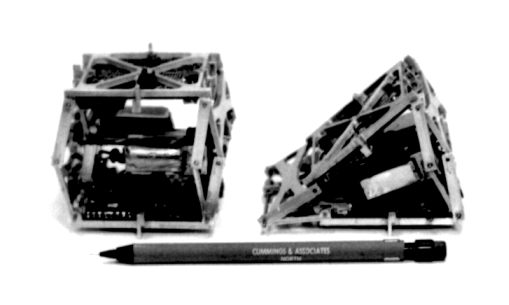
\includegraphics[width=\textwidth]{images/State_art_PolyPod.png}
                \caption{PolyPod segments}
                \label{fig:state_art_polypod-01}
        \end{subfigure}%
        ~ 
        \begin{subfigure}[b]{0.3\textwidth}
                \centering
               	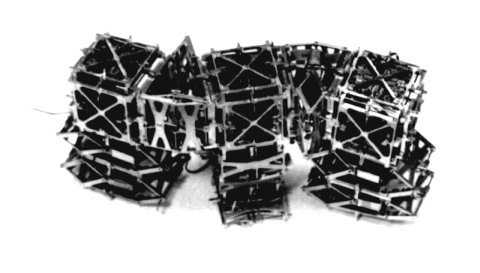
\includegraphics[width=\textwidth]{images/State_art_PolyPod-2.png}
                \caption{Robot made of PolyPod modules}
                \label{fig:state_art_polypod-02}
        \end{subfigure}
        \caption{PolyPod}
        \label{fig:state_art_polypod}
\end{figure}
%%%% polyBot %%%%%%%%%%%%%%%%%%%%%%%%%%%%%%%%%%%%%%%%%%%%%%%%%%%%%%%%%%%%
\subsection{PolyBot}
\label{state_modules_PolyBot}

\begin{figure}
        \centering
        \begin{subfigure}[b]{0.3\textwidth}
                \centering
                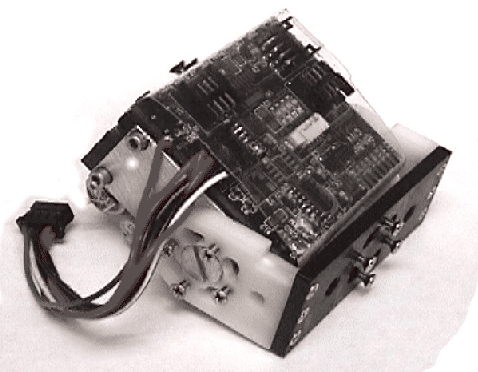
\includegraphics[width=\textwidth]{images/PolyBot_G1v4.png}
                \caption{G1v4}
                \label{fig:G1v4}
        \end{subfigure}%
        ~ 
        \begin{subfigure}[b]{0.3\textwidth}
                \centering
               	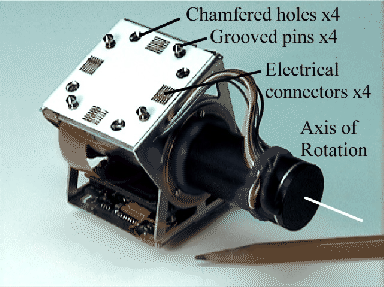
\includegraphics[width=\textwidth]{images/PolyBot_G2.png}
                \caption{G2}
                \label{fig:G2}
        \end{subfigure}
        ~
        \begin{subfigure}[b]{0.3\textwidth}
                \centering
                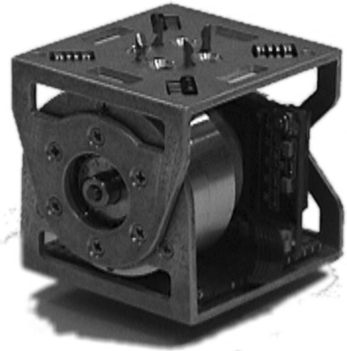
\includegraphics[width=0.8\textwidth]{images/PolyBot_G3.png}
                \caption{G3}
                \label{fig:G3}
        \end{subfigure}
		\caption{Three generations of PolyBot modules}\label{fig:PolyBot}
\end{figure}

PolyBot\cite{yim_modular_2003} is a modular robot developed by Mark Yim at the Palo Alto Research Center (PARC), as the evolution of the PolyPod robot. It has been designed with space missions in mind, resulting in a small and light module. It is currently formed by G3 modules, which are the third generation of modules developed for PolyBot. 
\\

The first generation modules were simple modules with one degree of freedom made from laser cut plastic with genderless symmetric passive connectors joined by screws, and a hobby servo for joint motion. They were not able of self-reconfiguration and the power and computations were given externally.
\\

The second generation modules were made from laser cut stainless steel, and the joint was actuated through a brushless motor that laid partially outside the module body due to the size of the gearbox. The connector was also upgraded with IR sensors and shape-memory alloy actuators for self-reconfiguration and active attachment/detachment. Communication among modules was carried through two CAN buses.
\\

For the third generation of modules, a smaller custom made gearbox was added to the brushless motor so that it would be contained inside the module. Power consumption was reduced and several improvements were introduced to the connectors, allowing them to make passive connections and increasing the IR accuracy.
\\


%%%% Conro %%%%%%%%%%%%%%%%%%%%%%%%%%%%%%%%%%%%%%%%%%%%%%%%%%%%%%%%%%%%%%
\subsection{CONRO}
\label{state_modules_CONRO}

\begin{figure}[b]
	\centering
	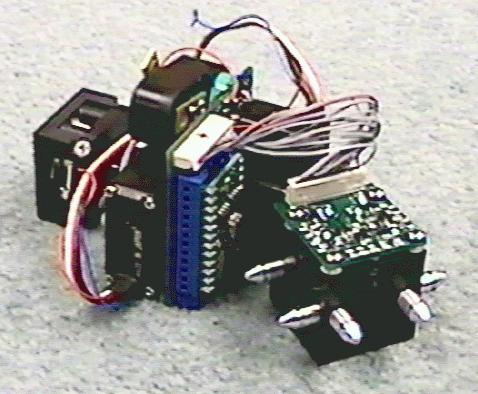
\includegraphics[width=0.3\textwidth]{images/CONRO01.jpg}
	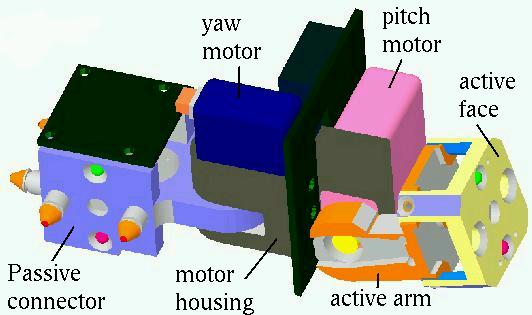
\includegraphics[width=0.3\textwidth]{images/CONRO02.jpg}
	\caption{CONRO module}\label{fig:conro}
\end{figure}
CONRO\cite{castano_conro_2002} is a self-reconfigurable robot developed at the University of Southern California with search, rescue and surveillance operations in mind. The modules for the CONRO robot are fully autonomous, and are divided into three main sections: a passive connector, an active connector and the main body. 
\\

The passive connector is a plastic cube with a pair of pins in three of its faces. These pins are made from aluminium and have a cylindrical shape, with a groove to allow the active connector to lock them. The passive connector is hollow, and holds two 160mAh lithium batteries of 3V and 6V and the IR serial communication trasmitters, receivers and control circuitry, which allows the module to communicate with its neighbours when connected and also in the docking process. The IR system also works as a position feedback information to position the modules correctly while docking.
\\

The main body holds two hobby servo which are connected with the passive and active connectors respectively and provide two degrees of freedom for the module. The body also contains the control board, which as a zero insertion force socket that allows the module to use three different microprocessors depending on the task requirements: a Stamp II based on a PIC16C57 or a Stamp IIe or II-SX based on a SCENIX SX28AC/SS processor.
\\

Finally, the active connector is equipped with a pair of holes for the passive connector pins and a latch for holding the modules together. Connection of the two modules is passive, whereas a shape-memory allow wire allows the disconnection of the module.


%%%% Superbot %%%%%%%%%%%%%%%%%%%%%%%%%%%%%%%%%%%%%%%%%%%%%%%%%%%%%%%%%%%
\subsection{Superbot}
\label{state_modules_Superbot}

\begin{figure}[h]
	\centering
	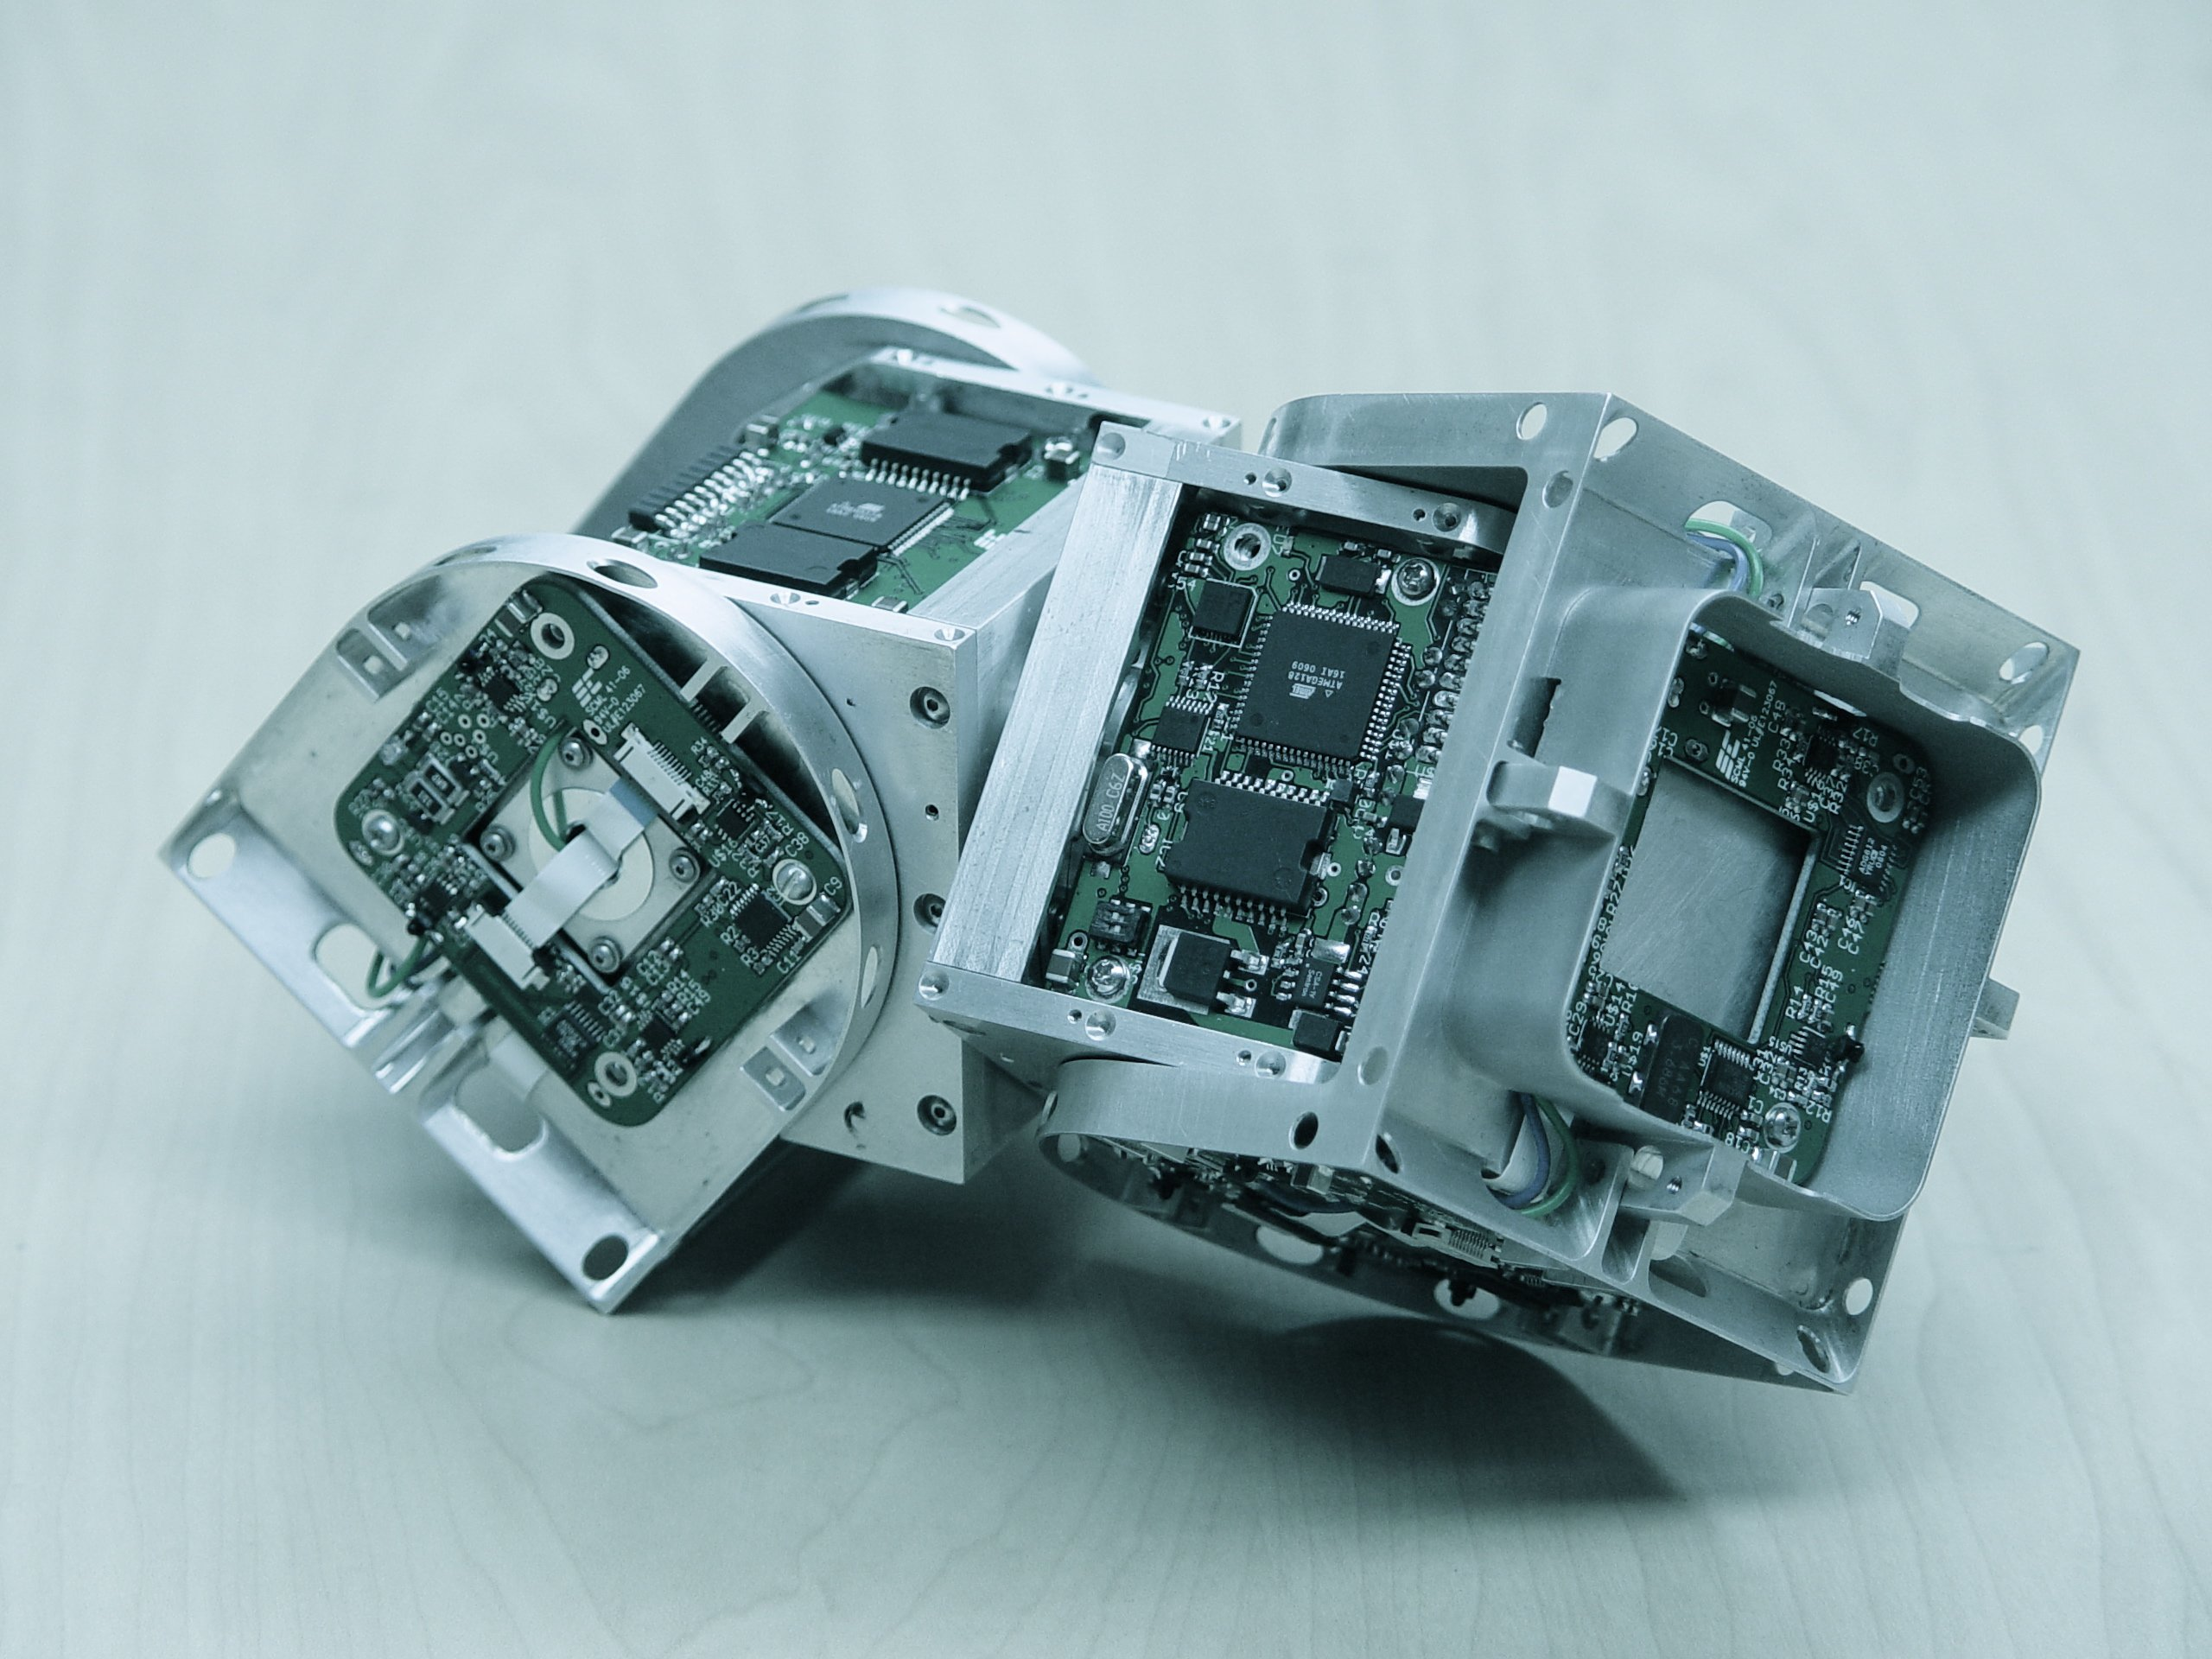
\includegraphics[width=0.3\textwidth]{images/Superbot01.JPG}
	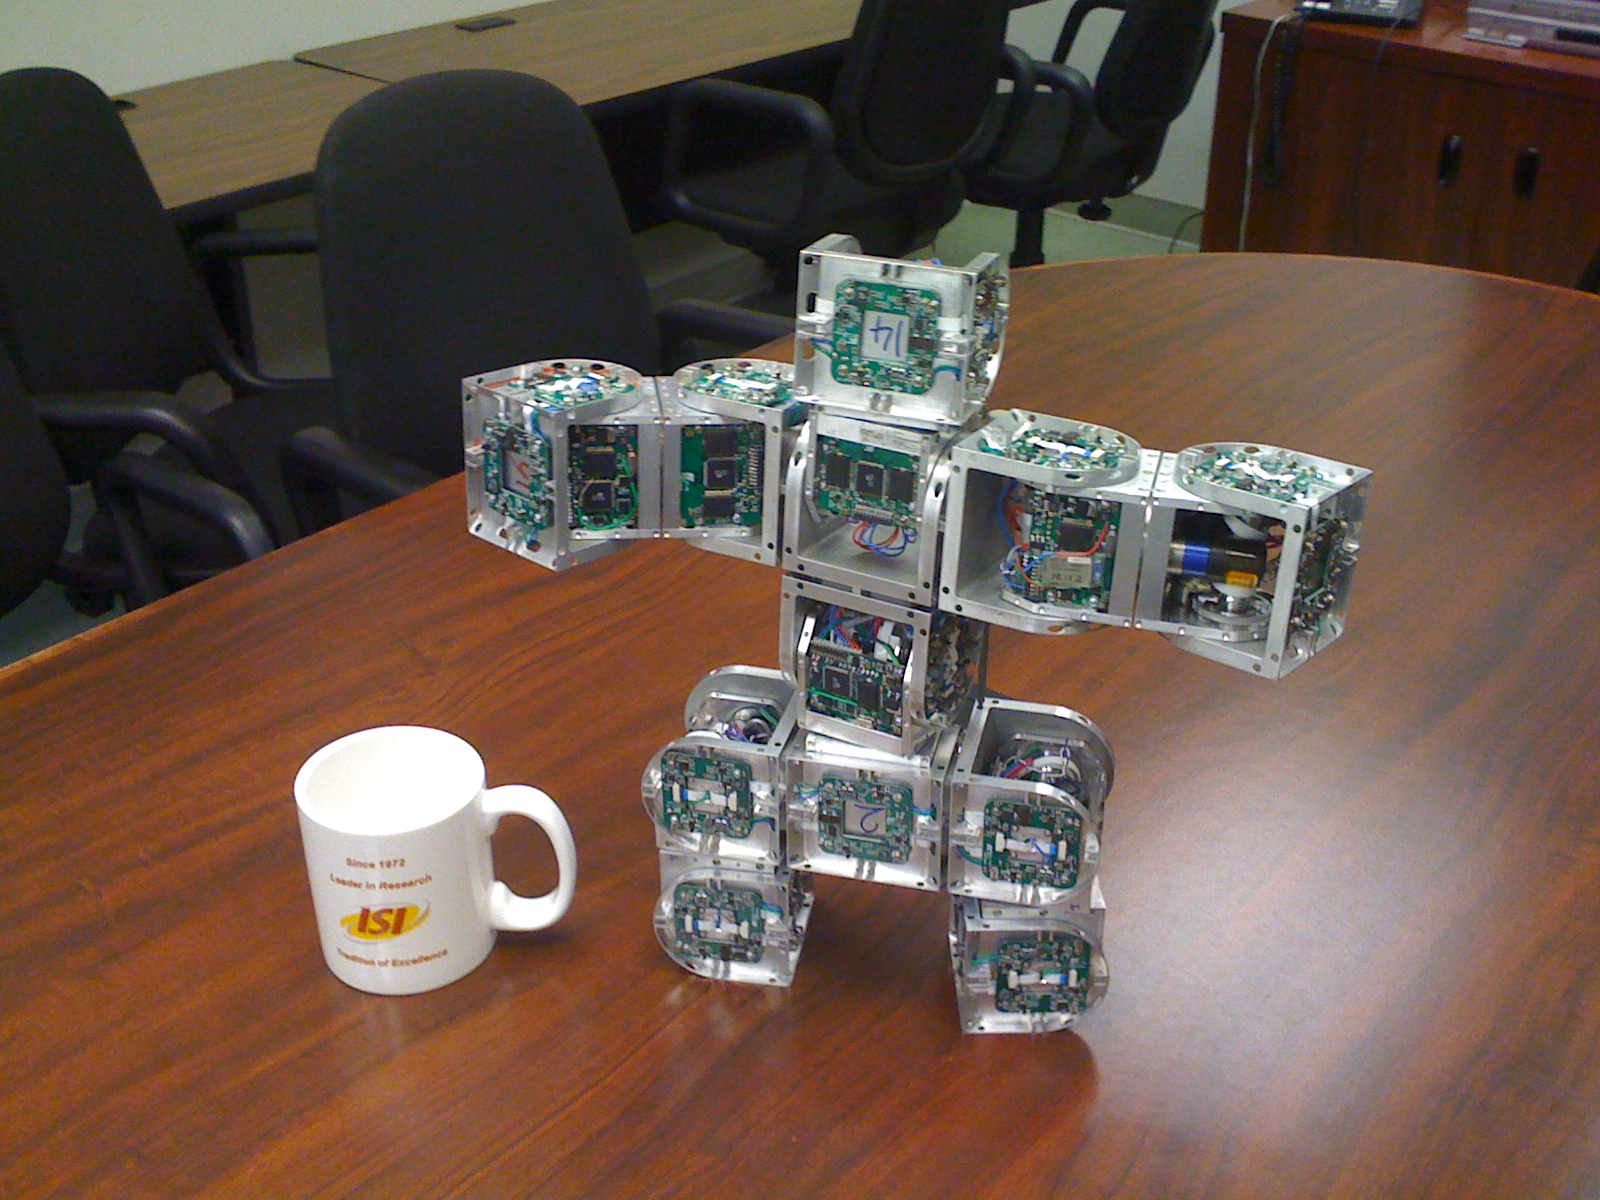
\includegraphics[width=0.3\textwidth]{images/Superbot02.JPG}
	\caption{Superbot module}\label{fig:superbot}
\end{figure}


The Superbot\cite{salemi_superbot:_2006} modular robot is the descendant of the CONRO module, and has been developed by the Polymorphic Robotics Laboratory at the University of Southern California. Funded by the NASA to be used for space applications, it is a hybrid module, as it can perform as a chain-type module or a lattice-type module.
\\

Superbot modules are made from two cube-like bodies of 84x84x84mm that have each one a degree of freedom. The joint between both cubes can rotate about 270º so it has a total of three degrees of freedom, which allows the module to move freely on a plane.
\\

Each degree of freedom is actuated by a DC motor equipped with a planetary gearbox and an external gearbox, and controlled by a software PID which recieves the feedback information from a potentiometer coupled to the motor shaft.
\\

The electronics design is modular and the main circuitry is divided into two boards, a master board on one half of the module, and a slave board on the other half. Each board has an ATmega128 microcontroller and both are connected through a I2C bus. Each one of the six connectors of the module has an IR communication system that allows communication with it neighbors and provide position and distance feedback for docking with other modules. 
\\

Power is supplied to the module by a 1600mAh, 7.4V lithium-polymer battery, and can be shared to the neighboring modules when needed through the connectors. This sharing process is controlled as a high-level routine by the microcontroller that manages this functionality.
\\

%%%% M-TRAN %%%%%%%%%%%%%%%%%%%%%%%%%%%%%%%%%%%%%%%%%%%%%%%%%%%%%%%%%%%%%
\subsection{M-TRAN}
\label{state_modules_M-TRAN}

\begin{figure}[t]
	\centering
	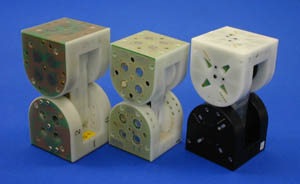
\includegraphics[width=0.3\textwidth]{images/M-TRAN01.jpg}
	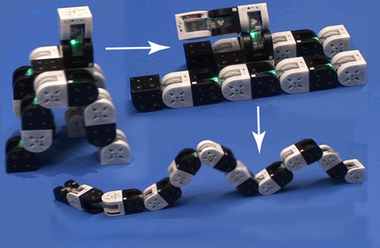
\includegraphics[width=0.3\textwidth]{images/M-TRAN02.jpg}
	\caption{M-TRAN module}\label{fig:m-tran}
\end{figure}

M-TRAN (Modular TRANsformer) \cite{murata_m-tran:_2002,kurokawa_m-tran_2003,kurokawa_distributed_2008} is a self-reconfigurable robot being developed by AIST and Tokyo-Tech since 1998. Their third and latest iteration of the robot is called M-TRAN III. M-TRAN is a hybrid module able to perform as a lattice-type modular robot for reconfiguration and as a chain/tree type for displacement.
\\

The module is made from two semi-cylindrical boxes and a link joining them together. One of these boxes is active, and has three connectors with hooks that are able to connect with the passive box of the other modulues. This design improves the previous one (used in M-TRAN and M-TRAN II) that used permanent magnets for connection and a shape-memory alloy coil for detachment, as it is several times faster (around 5 seconds for M-TRAN III system versus nearly 1 minute for the previous systems). Each box is able to rotate 180º around its joint with the link, giving M-TRAN a total of 2 parallel degrees of freedom. While in lattice mode, this joints are actuated only in multiples of 90º, allowing a checkerboard pattern in which active connectors coincide with passive connectors for reconfiguration.
\\

For the robot control, M-TRAN has four microcontrollers in total: one as master, that carries the main high-level behaviour and three slaves, that are in charge of several subsystems as the motor control, the communication system or sensors like the 3-axis accelerometer. It has several communication methods, such as bluetooth, IR and even a physical CAN bus through some pins on the connectors, which allows the modules to communicate no matter if they are physically in contact or in different assemblies.
\\

A battery and a power supply circuit are placed in the passive box of the M-TRAN module, supporting autonomous operation.



%%%% Y1 %%%%%%%%%%%%%%%%%%%%%%%%%%%%%%%%%%%%%%%%%%%%%%%%%%%%%%%%%%%%%%%%%
\subsection{Y1}
\label{state_modules_y1}


\begin{figure}[b]
		\centering
        \begin{subfigure}[b]{0.3\textwidth}
                \centering
                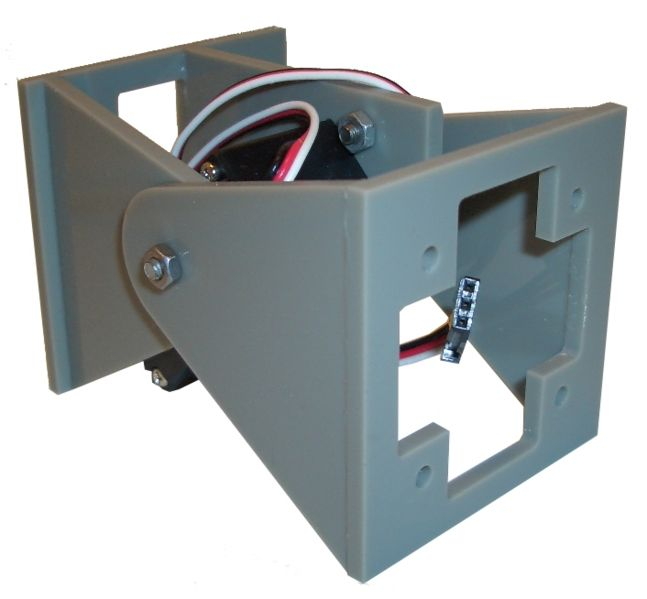
\includegraphics[width=\textwidth]{images/Y1_01.jpg}
                \caption{Y1}
                \label{fig:state_art_y1_mod}
        \end{subfigure}
        ~
        \begin{subfigure}[b]{0.3\textwidth}
                \centering
                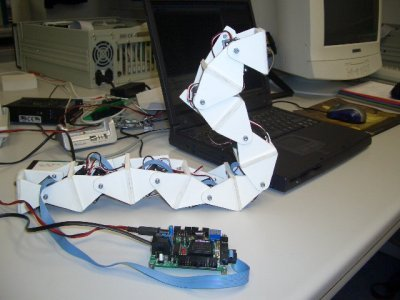
\includegraphics[width=\textwidth]{images/State_art_Y1_cube.jpeg}
                \caption{Cube Revolutions (Y1 snake)}
                \label{fig:state_art_y1_cube}
        \end{subfigure}
        \caption{Y1} \label{fig:state_art_y1}
\end{figure}

Y1\cite{gonzalez-gomez_website:y1} modules were developed by Juan Gonzalez-Gomez at the Autonomous University of Madrid based on the first generation of PolyBot modules. The main objective of the Y1 modules was to create a cheap and open platform for researching modular robotics.
\\

The Y1 modules are composed of a cheap hobby servo and a two-part housing made from laset cut PVC. This modules can be connected in a linear configuration, either pitch-pitch or pitch-yaw, allowing the resulting robots to move in a plane. Reconfiguration has to be done by hand, as the modules are joined by means of screws. The control electronics and the power source are supplied off-board.
\\

The Y1 module is open source hardware, which means that the plans, the files for manufacturing and the assembly instructions are available online for anyone to access to them. 
\\

The REPY-2.1 module developed by us and used for testing the gaits of this thesis is based on the Y1 module. More details about the Y1 and REPY-2.1 modules can be found in chapter \ref{hardware_chapter}.



%%%%%%%%%%%%%%%%%%%%%%%%%%%%%%%%%%%%%%%%%%%%%%%%%%%%%%%%%%%
%%%%%%%%%%%%%%%%%%%%%%%  GAITS  %%%%%%%%%%%%%%%%%%%%%%%%%%%
%%%%%%%%%%%%%%%%%%%%%%%%%%%%%%%%%%%%%%%%%%%%%%%%%%%%%%%%%%%
\section{Gait Generation on Modular Robots}
\label{state_art_controllers}

The lower level control for locomotion in mobile robots with wheels or tracks is usually not complicated, since it only involves turning the motors in order to produce movement. Difficulties appear at the higher level control, such as motion planning or navigation.\\

But, when the robot is articulated, either with legs or apodal, the lower level control becomes more complicated, as the problem of coordination appears, even if the robot is to travel through a flat surface without any kind of obstacles. In this kind of robots the movement of each of the joints must be coordinated with the movement of the other joints so that the robot can move. In more formal terms, the coordination problem can be stated as follows: \emph{For a robot with N articulations, find the value of each joint as a function of time $\varphi_i(t)$ so that the robot can achieve locomotion}. The solution of this problem is not unique, and depends on the type of gait that one desires to obtain (e.g. walking on a straight line, turning, trotting, galloping, etc).\\

In order to solve this problem, several approaches can be found in the literature, and they will be explained in this section.\\

\subsection{Gait tables}
\label{gait_gaittables}

Gait tables are tables that include the joint position values for each module at different steps of a gait. For each moment of the gait, each of the modules look up in the table what is the required joint value for the current step, and move their joints to that value. When the robot arrives at the end of the table, it starts again with the first position of the table, achieving a repeating pattern.\\

This is an easy and simple way to implement locomotion gaits for modular robots, and was first used by Mark Yim in his PolyPod \cite{Yim1993}. When the robots are composed of few modules and the desired movements are simple, these gait tables can be formed by hand, allowing a fast exploration of possible gaits for locomotion, as well as detecting mechanical defects on robot prototypes. Gait tables are not only useful for designing gaits for modular robots, but they can also be applied to other types of robots, such as quadruped, hexapods or even humanoid robots.\\

The main disadvantage of gait tables is that they lack flexibility, as for generating new gaits, or variations of the existing gaits, a new control table has to be created.\\

\subsection{Central Pattern Generators (CPGs)}
\label{gait_cpgs}
Central pattern generators (CPGs) are biological neural networks capable of producing coordinated patterns of rhythmic activity without any rhythmic inputs from sensory feedback or from higher control centers \cite{Ijspeert2008}. They are in charge of many rhythmic behaviours in both vertebrate and invertebrate animals, such as breathing, locomotion, bowel movements, etc.\\

CPGs are distributed networks composed by multiple coupled oscillatory centers, as observed in experiments with lampreys and salamanders, in which small sections of their spinal cords were capable of producing rhythmics activity. The lamprey is one the vertebrates most used to study CPGs, because its spinal column is transparent, contains few cells, and lasts at least a week outside
of the animal (in a saline solution) without deterioration \cite{Rovainen1979}, easing the work of the biologists.\\

Sensory feedback is not needed for the generation of the rhythms, but plays a key role in shaping the rhythmic patterns and keeping the body movements and the CPG coordinated. This coupling is so tight that is posible to induce CPG activity mecanically moving the tail of a lamprey, and to induce a normally looking walking gait in a decerebrated \footnote{Decerebration is the elimination of cerebral brain function in an animal by removing the cerebrum, cutting across the brain stem, or severing certain arteries in the brain stem \cite{decerebration}.} cat by placing it on a treadmill. If the treadmill is accelerated, the gait can even change from trot to gallop.\\

The complex locomotion behaviour generated by the CPG circuits is controlled by simple signals, that in many vertebrates are generated in a specific region of the brain stem known as \emph{Mesencephalic Locomotion Region} (MLR). Some experiments with electrical stimulation of this region have shown that the level of stimulation can modulate the speed of locomotions, and induce an automatic gait transition (from walk to trot to gallop on derebrated cats, and from walk to swimming on decerebrated salamanders). Therefore, basic rhythmic patters are generated at the spinal CPGs, but the modulation of those patterns according to environmental factors is controlled by the higher-level centers, such as the motor cortex, cerebellum and basal ganglia.\\

These biological CPGs have been matematically modelled as differential equations, and successfully applied to different robots, such as the \emph{Salamandra Robotica}, a salamander-like robot developed at the EPFL \cite{Ijspeert2007}. Since CPGs are a distributed approach, it has been also applied to modular robots, such as YaMoR \cite{Marbach2005} or the Roombots \cite{Sprowitz2010}. One advantage of using CPGs is that the transition between two steady state oscillations is bounded, continuous and relatively smooth, so if we are implementing an optimization algorithm for the gaits, and we randomly change the control parameters, the joint values will not change too abruptly, which helps preventing the motors from breaking \cite{Ijspeert2008}.\\

\subsection{Sinusoidal Oscillators}
\label{gait_sin_osc}

CPGs are very powerful, but they are complex and require lots of computing power. For that reason some researchers tried to substitute on their controllers the CPG model obtained by neurocomputing scientists by a simpler one that performs in a similar way, but using less resources. CPGs behave as fixed frequency oscillators in steady state, making sinusoidal oscillator a suitable canditate for being used as gait generators, as they are much simpler to model and require less resources for their implementation than CPGs. Implementations of sinusoidal oscillators have been tested successfully on snake robots by Lipkin et al., who also defined piecewise functions to perform specialized tasks, such as stair climbing \cite{Lipkin2007}, and Gonzalez-Gomez \cite{Gonzalez-Gomez2008}, who also studied the minimal configurations required for locomotion with sinusoidal oscillators \cite{Gonzalez-Gomez2006}. Sinusoidal oscillators also been applied to legged robots such as the hexapod robot Melanie-III with success \cite{AlonsoPuig2005}.\\

Other approaches simplify even more the coupled oscillators of the CPG approach, substituting them by a single sinusoidal waveform as a function of time and current module, that is used to control the all the joint positions \cite{Tesch2009}.\\

Due to its simplicity, sinusoidal oscillators are the approach selected in this thesis to solve the coordination problem, and are described in detail in chapter \ref{config_gait}.\\

\section{Coordination and Communications on Modular Robots}
\label{state_art_coordination}

Communication between robots is essential for achieving coordination. This becomes of special importance when working with modular robots, as because of their nature, they require their modules to colaborate with each others to complete a task. In order to achive reconfiguration or locomotion the modules need to know what their positions inside the modular robot are, what tasks or steps have been completed and which remain still pending for completion. \\

On modular robots, these communications are implemented on hardware in very different ways. Some of them, such as PolyPod, M-TRAN or SYMBRION / REPLICATOR have physical connectors that are used for communication when two modules are attached together \cite{Yim2000, Kurokawa2008, Liedke2011}, whereas most of the existing modules, such as CONRO, SUPERBOT or ATRON, communicate using IR or IrDA communications \cite{Castano2000, Salemi2006, Brandt2007}, which have the advantage of being wireless and that can be also used as distance sensors. A few modules, such as YaMoR or M-TRAN, can communicate using Bluetooth communications, allowing modules that are not physically attached to interact with each other\cite{ Mockel2006, Kurokawa2008}.\\

Communications between robots can be classified as global or local communications. In local communications, robots only talk to their nearest neighbors and information is shared locally. This approach is tipically used in modular robotics to find the topology of the robot and to coordinate local tasks. On the other hand, when using global communications all modules can communicate between each other and achieve coordination of tasks involving distant modules.\\

The type of communications a certain module can perform conditions its control strategy, modules with a global communication system usually apply centralized control methods, such as PolyPod's central gait tables\cite{Yim2000} or M-TRAN's centralized central pattern generators\cite{Kamimura2005} whereas modules with local communications tipically use distributed control methods, like CONRO's and SUPERBOT's distributed digital hormones \cite{Shen2002}.\\

Local communication methods are used mainly for coordination of reconfiguration in lattice-type modular robots and for coordination and synchronization of locomotion movements in chain-type modular robots. Butler et al. described a renconfiguration method for lattice modular robots using only local information based on cellular automata, a simple set of rules that control the reconfiguration steps depending on the neighbors attached to the module, and on the obstacles detected, allowing a flow-like locomotion\cite{Butler2004}. Funiak et al. presented a distributed method for module location inside large modular robots, consisting in breaking the cluster of modules in smaller clusters using normalized cut to identify dense sub-regions with small mutual localization errors\cite{Funiak2009}.\\

For locomotion synchronization and coordination the most notable distributed approach is digital hormones. Digital hormones are a nature-inspired communication method published by Shen et al., based on biological hormones, that consist on signals or messages that are propagated by the modular robot, triggering different actions depending on the function of the module that receives them. Those local actions are executed by the modules without the help of the hormone, and include joint movement and hormone manipulation and destruction, among others \cite{Shen2000}.\\

For this thesis digital hormones were selected as communication method due to their proved usefulness in distributed control of locomotion in chain-type robots \cite{Shen2002, Hou2006}. Digital hormones and our developed algorithm will be described in detail on chapter \ref{hormones}.\\
